\documentclass[12pt,a4paper]{article}
\usepackage{amsmath}
\usepackage{mathtext}
\usepackage{icomma}
\usepackage{amsfonts}
\usepackage{amssymb}
\usepackage[utf8]{inputenc}
\usepackage[T1,T2A]{fontenc}
\usepackage[english, russian]{babel}
\usepackage{graphicx}
\usepackage[left=2cm,right=2cm,top=2cm,bottom=2cm]{geometry}
\usepackage{calc}
\usepackage{wrapfig}
\usepackage{setspace}
\usepackage{indentfirst}
\usepackage{subfigure}
\usepackage[table,xcdraw]{xcolor}
\usepackage{float}
\usepackage[unicode, pdftex]{hyperref}
\usepackage{amsmath,bm}


\title{Гравитационное линзирование.\\
Оценка массы линзы в системе SDSS J0029-0055} 

\author{Исламов Сардор, группа Б02-111}

\begin{document}

\begin{titlepage}
    \centering
        {\bfseries 
        Министерство образования и науки Российской Федерации \\
        Московский физико-технический интститут \\
        (национальный исследовательский университет)}
        \vspace{3em}

        Физтех-школа физики и исследований им. Ландау
        \vspace{3em}         
    
        Отчет по проекту\\
        Компьютерные технологии решения научных задач
        \vspace{7em}
    
        \Large Гравитационное линзирование\\
        Оценка массы линзы в системе SDSS J0029-0055
    
        \vspace{5em}
    
        
        \small
        \begin{flushright}
            Студенты группы Б02-111\\
            \vspace{1em}

            Исламов Сардор\\
            \url{https://github.com/meIonmusk} \\
            \vspace{1em}

            Петухова Ксения
        \end{flushright}

        \vspace{20em}
        Долгопрудный\\ 2023
\end{titlepage}

\subparagraph*{Аннотация.} В данной работе представлен алгоритм построения модели сильного гравитационного линзирования (далее ГЛ) с протяженным источником в приближении точечной линзы. 
На основе построенной модели и открытых астрофизических баз данных и существующих публикаций проанализирована ГЛ система SDSS J0029-0055, определена масса линзы в ней: $M = 1.29^{+0.04}_{-0.03} \cdot 10^{11} M_\odot$.

\section*{Теоретическое введение}
\subparagraph*{Гравитационное линзирование.}
Гравитационное линзирование – это отклонение траектории света от прямолинейной в гравитационном поле массивных объектов. 
Выделяют три класса этого явления.
\begin{itemize}
    \item Сильное гравитационное линзирование, вызывающее легко различимые искажения, такие как кольцо или крест Эйнштейна, дуги и множественные изображения.
    \item Слабое гравитацонное линзирование, вызывающее слабое искажение источников, которые находятся позади линзы. 
    Его можно зафиксировать только после статистического анализа объектов фона, что позволяет найти небольшое согласованное искажение их изображений. 
    Проявляется в небольшом растяжении изображения перпендикулярно направлению к центру линзы.
    \item Микролинзирование, которое не вызывает видимых искажений формы, но может временно увеличивать или уменьшать количество света от источника.
\end{itemize}

\begin{wrapfigure}{r}{0.4\linewidth}
    \centering
    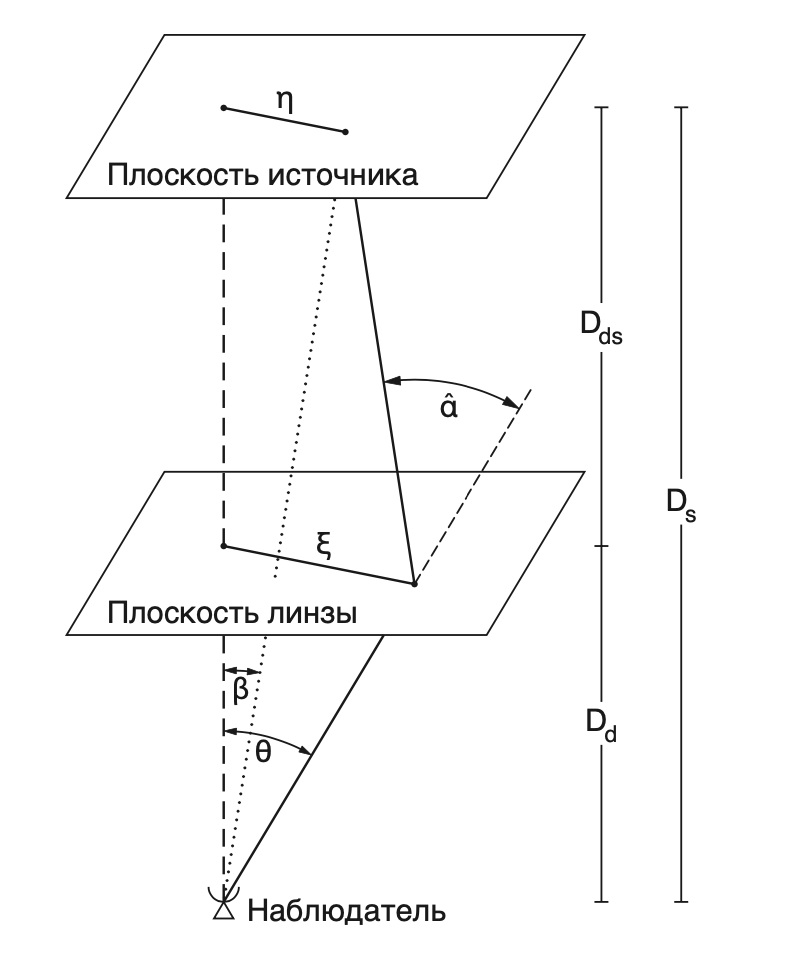
\includegraphics[width=\linewidth]{sources/scheme.png}
    \caption{\small{Схема гравитационного линзирования}}
\end{wrapfigure}  

\vspace{1em}
Здесь и далее речь пойдет о сильном гравитационном линзировании. 
В ходе линзирования преломление происходит на очень коротком участке траетории света. 
В реалистичных моделях линз, в которых масса, вызывающая линзирование, распределена трёхмерным образом, используется приближение плоских линз по аналогии с геометрической оптикой. 
Это всегда оправдано: характерные размеры самого большого объекта, который может быть линзой, - скопления галактик - порядка 1 Мпк, в то время как продольные расстояния между объектами системы порядка 100-1000 Мпк. 
Типичная гравитационно-линзированная система изображена на Рис. 1.

Углами $\bm{\beta}$ и $\bm{\theta}$ (двумерными векторами в соответствующих плоскостях) задаются положения источника света и его изображения соответственно. 
Уравнение линзы, описывающее отображение из плоскости источника на плоскость линзы:
\newline
\begin{equation}
    \bm \beta = \bm \theta - \alpha(\bm \theta) = \bm \theta - \frac{D_{ds}}{D_s} \widehat{\alpha}(\bm \xi)
\end{equation}

где $\alpha(\bm \theta)$ -- угол между положениями источника и его наблюдаемого изображения в плоскости линзы, $\widehat{\alpha}(\bm \xi)$ -- угол отклонения светового луча, $\bm \xi = D_d \bm \theta$ -- прицельный параметр, $D_d$, $D_s$ и $D_{ds}$ -- расстояния от наблюдателя до плоскости линзы, до источника и между плоскостями линзы и источника соответственно (см. Рис. 1)

Пусть масса линзы распределена в пространстве по закону $\rho(\bm \xi, z)$, где $z$ - координата вдоль оптической оси. 
Поверхностная плотность вещества в линзе задаётся следующим соотношением:

\begin{equation}
    \Sigma(\bm \xi) = \int \rho(\bm \xi, z) dz.
\end{equation}

Также вводится понятие критической плотности 
\begin{equation}
    \Sigma_{crit} = {c^2 \over 4 \pi G} {D_s \over D_d D_{ds}},
\end{equation}
где $c$ -- скорость света, $G$ -- гравитационная постоянная.
Радиус такой окружности в плоскости линзы, плотность внутри которой равна критической, называется радиусом Эйнштейна. 
Обычно он выражается в угловых единицах:

\begin{equation}
    \theta_E = \sqrt{{4 G  M \over c^2  } {D_{ds} \over D_d D_{s}}},
\end{equation}
где $M$ -- масса линзы. Эта величина характеризует масштабы гравитационного линзирования и является основной шкалой расстояний при описании этого явления.

Гравитационное линзирование сопровождается усилением интенсивности - важным явлением, без которого многие далекие объекты могли бы быть не обнаружены.
При этом само усиление ($magnification$) численно равно отношению суммарной площади изображений к видимой площади источника.
Для циркулярно симметричной линзы это значение равняется
\begin{equation}
    \mu = {\theta \over \beta}{ d\theta \over d\beta}.
\end{equation}

\subparagraph*{Точечная линза.}
Для сильного линзирования существует несколько основных приближений линз, призванных упростить теоретические выкладки.
Самыми простыми из них являются приближения точечной линзы и сингулярной изотермической сферы.

Далее будем рассматривать приближение точечной линзы с точечным источником.
В таком случае выражение для $\widehat{\alpha}(D_d \bm \theta)$ выглядит следующим образом:
\begin{equation}
    \widehat{\alpha}(\bm \xi) = {4 G M \over c^2 \xi^2} \bm \xi.
\end{equation}

\begin{wrapfigure}{r}{0.4\linewidth}
    \centering
    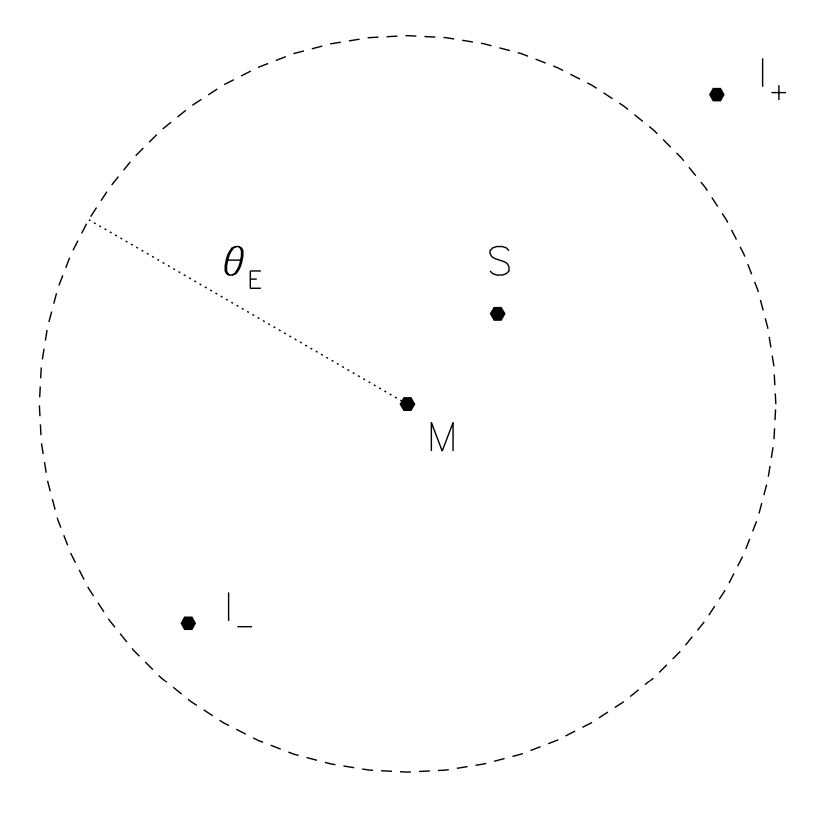
\includegraphics[width=0.8\linewidth]{sources/imagesForm.png}
    \caption{\small Относительные положения изображений $I_+$ и $I_-$, источника $S$ и линзы $M$ при гравитационном линзировании}   
\end{wrapfigure}

Тогда выражение (1) принимает вид 
\begin{equation}
    \bm \beta = \bm \theta - {4GM \over c^2 D_d \theta^2} {D_{ds} \over D_s} \bm \theta.
\end{equation}

Переходя к скалярным величинам и решая уравнение получаем следующие выражения:
\begin{equation}
    \theta_\pm = \frac 1 2 \left(\beta \pm \sqrt{\beta^2 + 4\theta_{E}^2}\right).
\end{equation}

Как видно, при $\beta \neq 0$ создается два изображения источника соответственно на расстояниях $\beta_-$ и $\beta_+$ от оси, проходящей через наблюдателя и линзу. 
При $\beta = 0$ изображение вырождается в кольцо Эйнштейна, радиус которого описывается выражением (4).

Для точечной линзы значение усиления представляется в следующем виде:
\begin{equation}
    \mu_\pm = \left[1 - \left({\theta_E \over \theta_\pm}\right)^4\right]^{-1} = {u^2 + 2 \over 2u\sqrt{u^2 + 4}} \pm \frac 1 2.
\end{equation}

\subparagraph*{Расстояние по угловому диаметру.} В космологии есть несколько способов определения расстояний. 
Для описания расстояний между объектами в системе источник - линза - наблюдатель используется понятие расстояния по угловому диаметру (angular diameter distance). 
Оно определяется следующим образом:
\begin{equation}
    D_A(z_1, z_2) = {1 \over 1 + z_2} \int_{z_1}^{z_2} {dz \over H_0\sqrt{\Omega_m (1+z)^3 + \Omega_\Lambda}},
\end{equation}
где $z_1$, $z_2$ -- красные смещения соответственно линзы и источника, вызванные расширением вселенной. 
В работе рассматривается плоская Вселенная с космологическими параметрами $H_0 = 70\ {\text{км} \over \text{с} \cdot \text{Мпк}},\ \Omega_m = 0.3,\ \Omega_\Lambda = 0.7$.

\subparagraph*{Построение модели.} Для расчета и анализа существующих систем напишем интерактивную модель для гравитационного линзирования.
Рассмотрим протяженные источники как совокупность точечных источников, линзирующихся одним массивным телом независимо друг от друга. 
Таким образом можно обобщить модель с точечной линзой и точечным источником на случай точечной линзы с протяженным источником.
Так как относительные расстояния между космическими телами велики, можем рассматривать все объекты находящиеся за линзой как далекий равноудаленный от нее фон.

Для качественного изображения и во избежание дефектов на нем также будем делать обратное преобразование вместо прямого -- для каждой точки можем однозначно определить, изображение какой точки исходного источника в ней должно находиться. 
Расчитывая для каждой вычисленной точки значения цвета пикселя и усиления, создаваемого линзой, получим сформированное линзированием изображение.

\subparagraph*{Посик системы.} 
\begin{wrapfigure}{r}{0.4\linewidth}
    \centering
    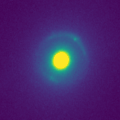
\includegraphics[width=0.7\linewidth]{sources/sdssj0029-0055.png}
    \caption{\small Изображение системы SDSS J0029-0055 в цветовой схеме viridis}
\end{wrapfigure}
Далеко не каждая система описывается рассматриваемым приближением точечной линзы: существует и множество других более сложных массивных объектов, как просто протяженных, так и вовсе не аксиально симметричных.
Процесс линзирования такими телами проходит сильно сложнее, и результаты отличаются от приведенных ранее выкладок.
По этой причине необходимо осуществить поиск системы, визуально подходящих под описанное приближение. 
Поиск систем и данных о них производился в открытых астрофизических базах данных, таких какс SIMBAD \cite{simbad}, архив изображений телескопа Hubble \cite{hubble}, каталог ESASky \cite{esasky}.

В целях анализа была выбрана система SDSS J0029-0055 (SDSS - Sloan Digital Sky Survey).
Для работы с ее изображением при помощи модуля $astropy$ на языке Python из найденного FITS-файла (Flexible Image Transport System) была вырезана часть с системой размером  $5'' \times 5''$.


\subparagraph*{Анализ изображений.}
Для анализа системы использовалась построенная модель. 
В качестве параметров были указаны красные смещения рассматриваемой системы $z_1 = 0.227$ и $z_2 = 0.9313$.

Для удобного сравнения реального изображения с полученными при моделировании создадим маску первого: значения пикселей с самими дугами, полученными в ходе линзирования, приравняем к единице, остальные занулим.
Подобрав подходящие положения в системе источник - линза в модели будем генерировать аналогичные изображения при разных массах. 
Для сравнения полученных изображений с маской, улучшим разрешение маски кубической интерполяцией. 
Теперь, имея изображения с одинаковым разрешением, определим количество несовпадающих пикселей. 
Построим график процента совпадения изображений в зависимости от массы линзы. 
Максимум будет соответствовать искомому значению. 
Погрешность определяется выбором отличия процента совпадения на $0.02\%$ от максимальной величины.

Вычисленные результаты можно видеть на Рис. 4
\begin{figure}[h]
    \centering
    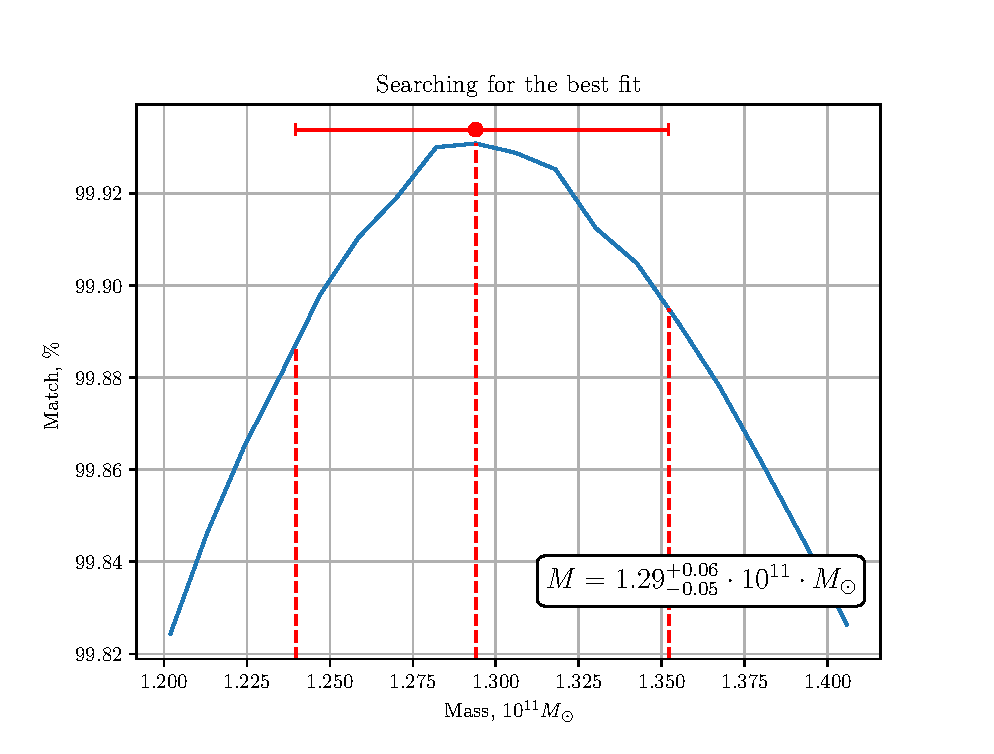
\includegraphics[width=0.8\linewidth]{sources/resultMass.eps}
    \caption{\small Поиск наилучшего совпадения модели с реальным изображением}
\end{figure}

\section*{Заключение}
В данной работе представлен алгоритм построения модели сильного гравитационного линзирования с протяженным источником в приближении точечной линзы. 
На основе построенной модели и открытых астрофизических баз данных и существующих публикаций проанализирована ГЛ система SDSS J0029-0055, определена масса линзы в ней: $M = 1.29^{+0.04}_{-0.03}\ M_\odot$.
Полученный результат хорошо согласуется с величиной, представленной в публикации Denzel et al. (2021) $M = 1.3^{+0.20}_{-0.22}\ M_\odot$.
Из этого можно заключить, что данная система хорошо описывается приближением точечной линзы.
Также этим подтверждается корректность построенной модели и ее приенимость для анализа реальных систем.

\newpage

\begin{thebibliography}{}
    \bibitem{gravlens_strong_weak_micro}
    \href{https://extras.springer.com/?query=978-3-540-30309-1}{P. Schneider, C.S. Kochanek, J. Wambsganss, Gravitational Lensing: Strong, Weak and Micro, 2006}
    
    \bibitem{meneghetti}
    \href{https://ui.adsabs.harvard.edu/abs/2022iglp.book.....M/abstract}{M. Meneghetti, Introduction to Gravitational Lensing (Lecture scripts)}

    \bibitem{narayan}
    \href{https://arxiv.org/abs/astro-ph/9606001}{R. Narayan, M. Bartellmann, Lectures on Gravitational Lensing}

    \bibitem{simbad}
    \href{http://simbad.u-strasbg.fr/simbad/}{SIMBAD Astronomical Database}

    \bibitem{hubble}
    \href{https://hla.stsci.edu/hlaview.html}{Hubble Legacy Archive}

    \bibitem{esasky}
    \href{https://sky.esa.int}{ESASky catalog}
\end{thebibliography}

\end{document}